\chapter{Experiments}\label{sec:experiments}

To inspect the potential benefits of self-supervised pre-training for \gls{ml}-based intrusion detection we chose to take a look at \gls{lstm} and Transformer networks as they are suited to process sequences of variable length and have shown promising results in the past \todo{give examples}. Network traffic data can be looked at from a multitude of perspectives ranging from aggregate statistical data over different time-frames \cite{kitsune} to looking at feature representations of single packets which can be viewed in the context of \textit{flows}. Flows are loosely defined as sequences of packets that share a certain property \cite{adversarial_recurrent_ids}. In our case we define flows as packets that share source and destination IP address, source and destination port, and the network protocol used. This creates the quintuple \textit{<srcIP, dstIP, srcPort, dstPort, protocol>} as the key over which individual packets are aggregated to flows. We used the data pre-processing from \cite{adversarial_recurrent_ids} as it fit the requirements for our experiments and was easily modifiable. The underlying data from which flow data is extracted are the \textit{CIC-IDS-2017} \cite{cic_ids_2017} and \textit{UNSW-NB15} \cite{unsw_nb15} \gls{nids} datasets. After the data pre-processing from \cite{adversarial_recurrent_ids} each packet is represented by source port, destination port, packet length, \gls{iat}, packet direction and all TCP flags (SYN, FIN, RST, PSH, ACK, URG, ECE, CWR, NS) resulting in 15 input features to be used in training the \glspl{nn}. \par

The task of the \glspl{nn} is to classify each flow into either \textit{benign} or \textit{attack} which results in a binary classification problem. Ordinary network traffic that should be ignored by the \gls{ids} is labeled as \textit{benign} and flows that constitute or are part of a cyber-attack are labeled as \textit{attack}. As there are only two possible labels, \gls{bce} can be used as loss function to determine the distance between the predicted label by the \glspl{nn} and the actual label \todo{give more detailed explaination of BCE Loss}. For updating weights we use the \textit{Adam} optimizer \cite{adam} which is an extension to the commonly used \gls{sgd} method. Similar to \textit{AdaGrad} \cite{optimizer_comparison} and \textit{RMSProp} \cite{optimizer_comparison} it maintains separate learning rates for each individual weight instead of using the same learning rate for every weight like in classic \gls{sgd}. Compared to other optimizers \textit{Adam} was shown to be more effective in improving training efficiency \cite{adam} and is appropriate for noisy or sparse gradients which can occur when working with \glspl{rnn} in general.

As a premise for our research we trained the \gls{lstm} and the Transformer network in a solely supervised fashion to get a baseline later results can be compared to. Supervised training was performed for 20, 100 and 500 epochs each for 90\%, 10\% and 1\% respectively of available data on both data-sets and a constant 10\% of data for validation which has not been used for training. A full overview of all experiments to establish a comparison baseline can be seen in \ref{table:experiments:baseline}. We specifically wanted to know how the networks would perform in a scenario where very little labeled training data was available as this would best describe a scenario where large amounts of unlabeled data are available for self-supervised pre-training and only a small amount of labeled data for fine tuning. To pre-train a \gls{nn} the network is given a task that is not necessarily connected to the final purpose of the network, often referred to as a \textit{proxy task}. By solving the proxy task the network attempts to find structure in the data and should learn to form a more abstract representation of the data within its latent space. E.g. with \gls{bert} pre-training is performed by masking a certain percentage of input tokens and having the \gls{nn} predict the missing words and additionally letting the network guess whether one sentences precedes another in a text. We defined our own proxy tasks for pre-training the networks as described in the following sections. Pre-training is performed with 80\% of available data, supervised fine-tuning with 1\% and validation with 10\% of data.

\begin{table}[h]
	\scalebox{0.92}{
		\begin{tabular}{c c c c c c}
			\textbf{Model} & \textbf{Dataset} & \multicolumn{1}{l}{\textbf{Batchsize}} & \textbf{Subset} & \textbf{Training \%} & \multicolumn{1}{l}{\textbf{Training Epochs}} \\ \hline \midrule
			LSTM           & CIC-IDS-2017     & 128                                     & - 		& 90                   & 40                                            \\ \midrule
			LSTM           & CIC-IDS-2017     & 128                                     & - 		& 10                   & 40                                            \\ \midrule
			LSTM           & CIC-IDS-2017     & 128                                     & - 		& 1                    & 200                                           \\ \midrule
			LSTM           & CIC-IDS-2017     & 128                                     & CIC\_10	& -                    & 600                                           \\ \midrule
			LSTM           & UNSW-NB15        & 128                                     & -			& 90                   & 40                                            \\ \midrule
			LSTM           & UNSW-NB15        & 128                                     & -			& 10                   & 40                                            \\ \midrule
			LSTM           & UNSW-NB15        & 128                                     & -			& 1                    & 200                                           \\ \midrule
			LSTM           & UNSW-NB15        & 128                                     & CIC\_10	& -                    & 600                                           \\ \midrule
			Transformer    & CIC-IDS-2017     & 512                                     & -			& 90                   & 40                                            \\ \midrule
			Transformer    & CIC-IDS-2017     & 512                                     & -			& 10                   & 40                                            \\ \midrule
			Transformer    & CIC-IDS-2017     & 512                                     & -			& 1                    & 200                                           \\ \midrule
			Transformer    & CIC-IDS-2017     & 512                                     & UNSW\_10	& -                    & 600                                           \\ \midrule
			Transformer    & UNSW-NB15        & 512                                     & -			& 90                   & 40                                            \\ \midrule
			Transformer    & UNSW-NB15        & 512                                     & -			& 10                   & 40                                            \\ \midrule
			Transformer    & UNSW-NB15        & 512                                     & -			& 1                    & 200                                           \\ \midrule
			Transformer    & UNSW-NB15        & 512                                     & UNSW\_10	& -                    & 600                                           \\
	\end{tabular}}
	\caption{List of baseline training runs used for comparison later in the thesis.}
	\label{table:experiments:baseline}
\end{table}

\section{Self-supervised Pre-training for Long Short-Term Memory Networks} \label{sec:experiments_lstm}

For our \gls{lstm} network we chose a three layer \gls{lstm} with a \textit{hidden size} and \textit{cell size} of 512. While a larger network might be slightly more effective, this configuration proved to be swiftly trainable while also producing results close to the optimum \todo{provide numbers}. Since we are only interested in comparisons between different training methods applied to the same model, it is not necessary to increase model size to achieve optimal results as this would unnecessarily increase the training time needed until the model converges. For training the \gls{lstm} model, each flow is considered one sample and each packet is one token. The tokens are processed by the model in chronological order, meaning packets with an earlier timestamp will be processed first. The timestamp however is not part of the feature representation but is considered for data pre-processing to order packets within flows. For pre-training the \gls{lstm} we devised five different proxy tasks for the model to solve in a self-supervised fashion: Predicting the next packet in the flow, predicting masked features of randomly chosen packets and predicting randomly masked packets, the identity function and an AutoEncoder. The \gls{mae} is used to determine the divergence between prediction and target data. Translating to PyTorch this means we used \textit{L1Loss} with \textit{mean} reduction as the loss function for pre-training. We tuned the hyper-parameters of training for both supervised and self-supervised training to an initial \textit{learning rate} of $10^{-3}$ and a \textit{batch size} of 128. Over the training process, the learning rate will be adjusted by Adam so the model is robust to changes on the initial learning rate. For every proxy task, the model has been trained with the different parameters in table \ref{table:experiments:lstm_proxy_tasks} to establish comparable results.

\begin{table}[bh]
	\scalebox{0.90}{
		\begin{tabular}{c c c c c c c c}
			\textbf{Model} & \textbf{Dataset} & \multicolumn{1}{l}{\textbf{B.s.}} & \textbf{Subset} & \textbf{Tr. \%} & \multicolumn{1}{l}{\textbf{Tr. Eps.}} & \textbf{Pretr. \%} & \textbf{Pretr. Eps.} \\ \hline \midrule
			LSTM           & CIC-IDS-2017     & 128                                     & -               & 10              & 40                                     & 80                 & 10                   \\ \midrule
			LSTM           & CIC-IDS-2017     & 128                                     & -               & 1               & 200                                    & 80                 & 10                   \\ \midrule
			LSTM           & CIC-IDS-2017     & 128                                     & CIC\_10         & -               & 600                                    & 80                 & 10                   \\ \midrule
			LSTM           & UNSW-NB15        & 128                                     & -               & 10              & 40                                     & 80                 & 10                   \\ \midrule
			LSTM           & UNSW-NB15        & 128                                     & -               & 1               & 200                                    & 80                 & 10                   \\ \midrule
			LSTM           & UNSW-NB15        & 128                                     & UNSW\_10         & -               & 600                                    & 80                 & 10                   \\ \midrule
	\end{tabular}}
	\caption{Training and pretraining configurations for \gls{lstm} model trainings with different proxy tasks.}
	\label{table:experiments:lstm_proxy_tasks}
\end{table}

\begin{itemize}
	\item different parameterization of LSTM
	\item two consecutive 3-layered LSTMs
	\item orthogonal initialization
	\item CrossEntropy Loss instead of BCE
\end{itemize}

\subsection{Identity Function} \label{sec:experiments_lstm_identity}

The simplest form of a proxy-task for pre-training is having the model learn the identity function.
In practice that means that input sequence $x^{(t)}$ and target sequence $y^{(t)}$ are the same $x^{(t)} = y^{(t)} = x^{(1)}, x^{(2)}, ... , x^{(n)}$ where $n$ is the sequence length. The model learns to convey the information through the network at each time step. For this task, the model does not need to derive any meaningful hidden representation of the data, but as our experiments show it still moves the weights of the model into a favorable direction when compared to a 0-initialization or an orthogonal initialization. 

\subsection{Predict Packet} \label{sec:experiments_lstm_predict_packet}

For this proxy task, the model has to predict the next packet in the flow. We started by predicting only the last packet in each flow but then moved to predicting all packets in a flow except the first. This means having a \textit{sequence-to-sequence} model where the inputs are all tokens in one flow with length $n$ except the last, because it has no successor: $x^{(t)} = (x^{(1)}, x^{(2)}, ..., x^{(n-1)})$. The target data are all tokens in the same flow except the first, because it has no predecessor: $y^{(t)} = (x^{(2)}, x^{(3)}, ..., x^{(n)})$. \glspl{lstm} process data in sequential order so at each time step, the model only has information of packets in the past and is to predict what the next packet in the flow will be. This results in two comparable tensors $y^{(t)}$ and the model output sequence $\hat{y}^{(t)} = (\hat{y}^{(1)}, \hat{y}^{(2)}, ..., \hat{y}^{(n-1)})$ of equal length $n-1$ between which a differentiable loss $C(y^{(t)},\hat{y}^{(t)})$ can be calculated. This way, a lot of information is conveyed to the network when compared to only predicting the last packet in a flow. At first glance, this looks similar to the identity function in \ref{sec:experiments_lstm_identity}. The key difference is however, that the token which is to be predicted is not yet available as an input token to the model, meaning it has to derive the features by other means than conveying the requested input token to the output. The loss is calculated as the \gls{mae} (\textit{L1Loss} with \textit{mean} reduction) between the predicted logits and the target data sequences.

\subsection{Mask Features} \label{sec:experiments_lstm_mask_feature}

For this pre-training task, the model is to predict masked features of some packets in the sequence. We have tried multiple masking values but -1 produces the best results out of the values we tried \todo{give a comparison of values}. This proxy task in particular can be parameterized in different ways. E.g. the number of features and which features to mask, if always the same features are masked or if the selection is random for each packet or for each flow, if every packet in the sequence has some masked features or if there is only a chance that a packet is selected for masking. Those are only some examples of how this task can be set up in different ways. To be completely exhaustive was not possible, so we compiled a selection of some of the variations as an overview of the parameter space. For pre-training the model is provided masked data as input sequence and the unmasked data is the target. The loss is calculated as the \gls{mae} (\textit{L1Loss} with \textit{mean} reduction) between the predicted \textit{logits} and the target data sequences. \todo{enumerate all parameter combinations used}

\subsection{Mask Packets} \label{sec:experiments_lstm_mask_packet}

Similar to the pre-training in \gls{bert}, all features of random packets in the sequence are masked with a value of -1 and the model is to predict the masked tokens. Again, \gls{mae} is used as the loss function. Unlike to \gls{bert}, we don't only look at the masked tokens when calculating the loss but compare every feature of every packet, also the non-masked ones, which adds an auto-encoding property to the pre-training. We found this to have more beneficial effect on the results than only looking at the masked packets. The most important parameter here is the ratio of how many packets per sequence are to be masked compared to its sequence length. To work with an absolute number of masked packets is not feasible as sequence length varies from 1 to a set max sequence length which in our case was 100. If an absolute number was used to determine how many packets should be masked some sequences would be completely masked out which would not be beneficial for training.

\subsection{Auto-Encoder} \label{sec:experiments:lstm_auto_encoder}

As explained in section \ref{sec:backgrund:autoencoder}, for the Auto-Encoder the model is tasked with compressing and decompressing the data as lossless as possible. With an \gls{lstm} model, this means having two consecutive \gls{lstm} models where the first is to encode the sequence and the second is to decode the sequence. As template we used the model proposed by Nitish Srivastava et al. in their paper "Unsupervised Learning of Video Representations using LSTMs" \cite{unsupervised_learning_lstms}, but similar proposals for Auto-Encoders with \glspl{lstm} can be found in \cite{unsupervised_learning_lstms_timeseries} or \cite{lstm_anomaly_detection}. \par
The encoder \gls{lstm} compresses the whole input sequence $x_e^{(t)} = (x_e^{(1)}, x_e^{(2)}, ..., x_e^{(n)})$ into the hidden state of the last stage $h_e^{(n)}$ ($C_e^{(n)}$) where $n$ is the length of the input sequence. The decoder \gls{lstm} is then initialized with the hidden and cell state of the last stage from the encoder \gls{lstm} $h_d^{(1)} = h_e^{(n)}, C_d^{(1)} = C_e^{(n)}$ trying to reconstruct the input sequence. After every stage of the decoder, either the output of the current stage $\hat{y}^{(t)}$ or the target token of the current stage $x^{(t)}$, the ground truth, is then fed into the model as input token  $x_d^{(t+1)} = \hat{y}^{(t)}$ for the next stage to calculate the next time step. The first input token for the decoder is a zero vector which functions as a start-of-sequence token $x^{(1)} = 0$. This way, the encoder is forced to store as much information about the sequence as possible in the hidden state and as the size of the hidden state is constrained, it has to find an abstract representation of the sequence. For supervised fine-tuning and validation, only the encoder part of the model is used. \todo{insert graphic}

\subsection{Composite model} \label{sec:experiments:lstm_composite}

For the composite model we recreated the network proposed by Nitish Srivastava et al. in their paper "Unsupervised Learning of Video Representations using LSTMs" \cite{unsupervised_learning_lstms} as summarized in section \ref{sec:stateofart:unsupervised_video_lstm}. As a self-supervised pre-training proxy task, the model is fed half the packet sequence of a flow and is tasked with both reconstructing the part of the sequence it had access to, and predicting the missing part of the flow which it had no access to. The output of the model is a sequence $\hat{y}^{(t)}$ of length equal to the original input sequence $x^{(t)}$ of which the first half is reconstructed and the second half is predicted by the model. The loss is again calculated as the \gls{mae} (\textit{L1Loss} with \textit{mean} reduction) between the original input and the output sequence of the model. The model consists of three \glspl{lstm} which can be labeled \textit{encoder}, \textit{decoder} and \textit{predictor} as can be seen in figure \ref{fig:experiments:unsupervised_lstm_composite}. The encoder processes the first half of the original input sequence, constructing an abstract representation in its hidden state. The hidden state of the last stage of the encoder \gls{lstm} is copied to both the decoder and predictor \glspl{lstm} as initial hidden state. Exactly like the Auto-Encoder from the previous section \ref{sec:experiments:lstm_composite} the decoder \gls{lstm} tries to recreate the input sequence. Initialized with the final hidden state of the encoder, the predictor \gls{lstm} tries foretell future packets of the flow. At every stage of the predictor \gls{lstm} (except the first), either the output $\hat{y^{(t-1)}}$ of the previous stage or the target token $x^{(t-1)}$ of the previous stage is used as input token for the next stage. The authors of \cite{unsupervised_learning_lstms} label those two methods \textit{conditioned} and \textit{uncondition} as is further explained in section \ref{sec:stateofart:unsupervised_video_lstm}.


\begin{figure}[h]
	\centering
	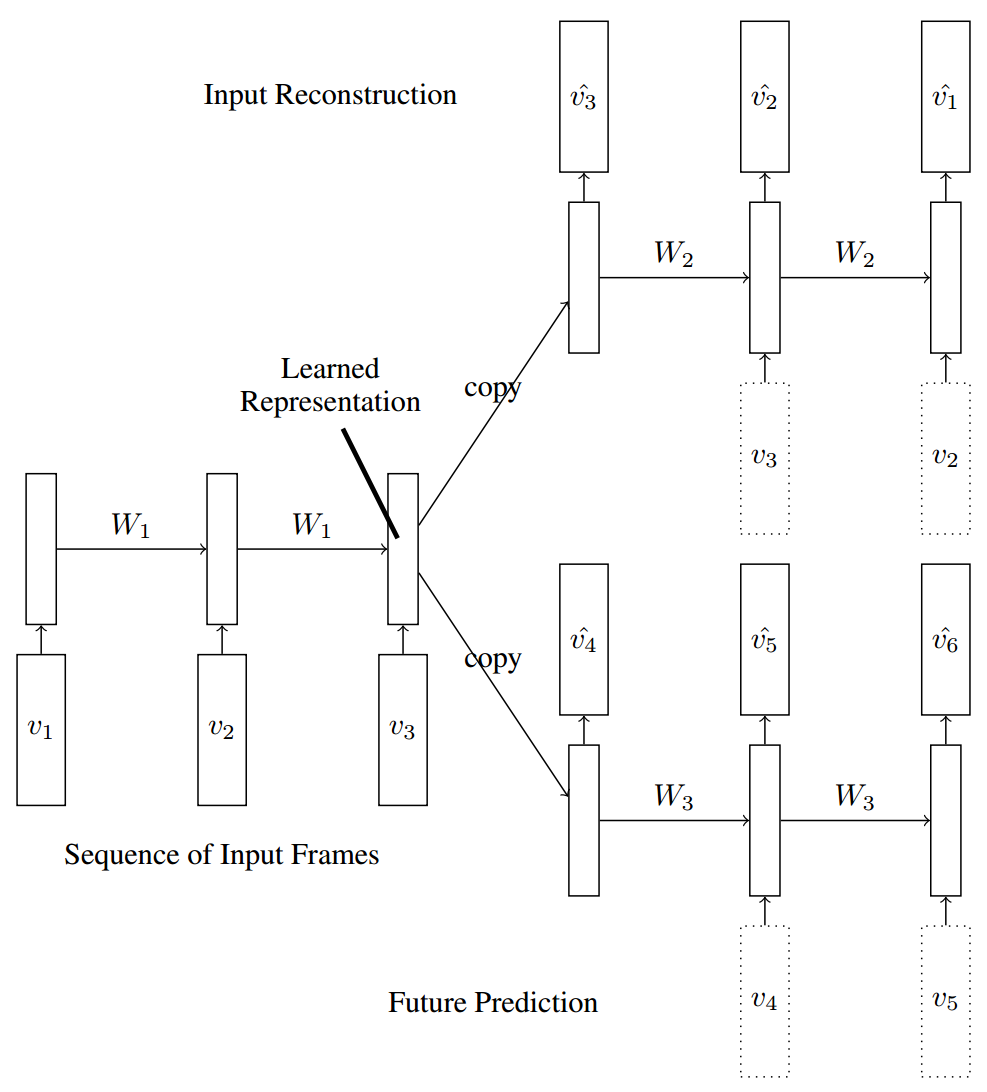
\includegraphics[width=0.7\textwidth]{img/unsupervised_learning_with_lstms_composite.png}
	\caption{Composite model for input reconstruction and future prediction \cite{unsupervised_learning_lstms}}
	\label{fig:experiments:unsupervised_lstm_composite}
\end{figure}	

\todo{make own graphic with labels encoder, decoder, predictor}

\section{Self-supervised Pre-training for Transformer Networks} \label{sec:experiments_transformer}

Following the example of \gls{bert} we only used the encoder part of the transformer since the decoder does not provide any benefit for classification problems. We tuned the model parameters to be 10 Transformer layers, each layer consisting of a 3-headed Multi-Head Attention block and a feed-forward network with a forward expansion of 20 times the input size, i.e. the number of features per packet. Since we did not observe any over-fitting during training, we set the drop-out rate to zero (except for training with the Auto-Encoder \ref{sec:experiments_transformer_autoencoder}). 
Like with the \gls{lstm} we devised a series of proxy tasks for pre-training the model in self-supervised fashion. Since the information flow is different in Transformers than it is in \glspl{lstm}, the pre-training task \textit{Predict Packets} \ref{sec:experiments_lstm} we used for the \gls{lstm} is no longer feasible. While the \gls{lstm} at each stage has only access to all the tokens it processed up to this point, the Transformer has access to all input tokens at each stage of the execution which is one of the benefits of self-attention \cite{attention}. Contrary to our expectations, supervised training (with 90\% auf the dataset) on the Transformer takes longer than on the \gls{lstm} to achieve the observed optimal accuracy of 99,65\%. In other words, when training the \gls{lstm} and the Transformer network with the same amount of data for the same amount of time, the \gls{lstm} produces better results. In the following sections we describe the pre-training methods we used to pre-train the Transformer network.

\begin{table}[h]
	\scalebox{0.86}{
		\begin{tabular}{c c c c c c c c}
			\textbf{Model} & \textbf{Dataset} & \multicolumn{1}{l}{\textbf{B.s.}} & \textbf{Subset} & \textbf{Tr. \%} & \multicolumn{1}{l}{\textbf{Tr. Eps.}} & \textbf{Pretr. \%} & \textbf{Pretr. Eps.} \\ \hline \midrule
			Transformer    & CIC-IDS-2017     & 512                                     & -               & 10              & 20                                     & 80                 & 10                   \\ \midrule
			Transformer    & CIC-IDS-2017     & 512                                     & -               & 1               & 100                                    & 80                 & 10                   \\ \midrule
			Transformer    & CIC-IDS-2017     & 512                                     & CIC\_10        & -               & 500                                    & 80                 & 10                   \\ \midrule
			Transformer    & UNSW-NB15        & 512                                     & -               & 10              & 20                                     & 80                 & 10                   \\ \midrule
			Transformer    & UNSW-NB15        & 512                                     & -               & 1               & 100                                    & 80                 & 10                   \\ \midrule
			Transformer    & UNSW-NB15        & 512                                     & UNSW\_10        & -               & 500                                    & 80                 & 10                   \\ 
	\end{tabular}}
	\caption{Training and pretraining configurations for Transformer model trainings with different proxy tasks.}
	\label{table:experiments:transformer_proxy_tasks}
\end{table}

\todo{write}

\begin{itemize}
	\item two consecutive TransformerEncoders, one for pre-training, one for fine-tuning
	\item Classification (CLS) Token
	\item Resetting last Layers 1,...,5 of Transformer after pre-training
	\item Use decoder also
	\item different dropout rates
	\item different number of attention heads
\end{itemize}

\subsection{Mask Features} \label{sec:experiments_transformer_mask_features}

Analogous to the \textit{Mask Features} proxy task for the \gls{lstm}, we used the same method for pre-training the Transformer.

\subsection{Autoencoder} \label{sec:experiments_transformer_autoencoder}

Autoencoder are an established concept when it comes to self-supervised learning \ref{sec:background:auto_encoder}. With this method input and target data are the same and the network is tasked with reconstructing the input data at the output. To prevent the network from simply "transporting" the input tokens through the network without having to learn anything, a form of regularization is introduced to force the network into learning an abstract representation of the data \cite{autoencoders}. 
In our case, we used the dropout rate to introduce artificial noise into the input data.

\subsection{Mask Packet}

For this proxy task, random packets in the flow are masked with a value of -1 and the model is to predict only the masked packets. Since a packet in a flow can be seen as a word in a sentence, and the feature representation of a packet is similar to an embedded word vector, this pre-training task is analogous to the method used in \gls{bert} \cite{bert}. 

\newpage
